\documentclass[report.tex]{subfiles} 
\begin{document}
\chapter{Implementation Details}
\label{chap:implementation details}
Approximately each section in chapter \ref{sec:theory} is translated into a separate VHDL component. Some components are in themselves also divided in subcomponents to make the code more manageable. The complete and most up-to-date code is found on \url{https://github.com/Risca/Fierce-Gravel}.

Since almost each operation in chapter \ref{sec:theory} is a separate component and the fact that the source code available on-line is well commented, this section will only highlight the topics of the VHDL implementation that require further explanation. These topics include:

\begin{itemize}
\item The \emph{Resources} package
\item The \emph{Variables} Package
\item Test Benches
\end{itemize}

\section{The \emph{resources} and \emph{variables} packages}
The VHDL standard defines an elegant way to summarize all different types, subtypes, functions, components, etc. in what is called a \emph{package}. This project have two packages for all its parts --- The \emph{resources} and the \emph{variables} package.

\subsection{\emph{Resources} package}
This package contains type and component declarations, and a few functions.

The type definitions were introduced to make it clear what signals the input and outputs of each component are supposed to be fed.
Listing \ref{list:typedefs} show the six different types used throughout the project.

\begin{figure}[ht]
\lstinputlisting[firstline=7,
                 firstnumber=7,
                 lastline=20,
                 label={list:typedefs},
                 caption={FG\_package.vhd, type definitions}]
{FG_package.vhd}
\end{figure}

The component declarations are not very informative to list here and the reader is therefore referred to the on-line source.

To be able to use the type definitions above, the XOR operator function had to be overloaded.

The round constant is also defined as a function, mainly because of simplicity.

Listing \ref{list:func dec} and listing \ref{list:func def} show the function declarations and definitions respectively.

%\begin{figure}[ht]
\lstinputlisting[firstline=151,
                 firstnumber=151,
                 lastline=156,
                 label={list:func dec},
                 caption={FG\_package.vhd, function declarations}]
{FG_package.vhd}
%\end{figure}

%\begin{figure}[ht]
\lstinputlisting[firstline=162,
                 firstnumber=162,
                 lastline=213,
                 label={list:func def},
                 caption={FG\_package.vhd, function definitions}]
{FG_package.vhd}
%\end{figure}

\subsection{\emph{Variables} package}
This package is not part of \emph{resources} mostly for convenience. I gathers all the constants and variables needed throughout the project, and can be seen in listing \ref{list:variables}

%\begin{figure}[ht]
\lstinputlisting[firstline=6,
                 firstnumber=6,
                 lastline=21,
                 label={list:variables},
                 caption={FG\_variables.vhd, Constants and variables used}]
{FG_variables.vhd}
%\end{figure}

\section{Test benches}

To facilitate testing of each component during this project, most components take at least a state\_array as an input and a state\_array as an output. Some components also accept a round\_key. This generalized input and output make it very easy to test each component, or even operator, individually.

Three test benches are pre-made in the online sources
\begin{itemize}
\item AES\_enc.vhd -- For testing the encryption and it's components, subcomponents and operators
\item AES\_dec.vhd -- For testing the decryption and it's components, subcomponents and operators
\item KeySchExp.vhd -- For testing the key expansion
\end{itemize}

The test benches have an input for selecting a few pre-programmed sets of input data. The data can be changed at compile-time. 

All test benches also have outputs for viewing the output data on the 7-segment displays on the Altera DE2 development board. The 7-segment displays can display one column (four bytes) at a time. Two switches are used to select which column of the output that should be displayed.

See figure \ref{fig:test bench overview} for a schematic overview on how the test benches work.

\begin{figure}[ht]
\centering
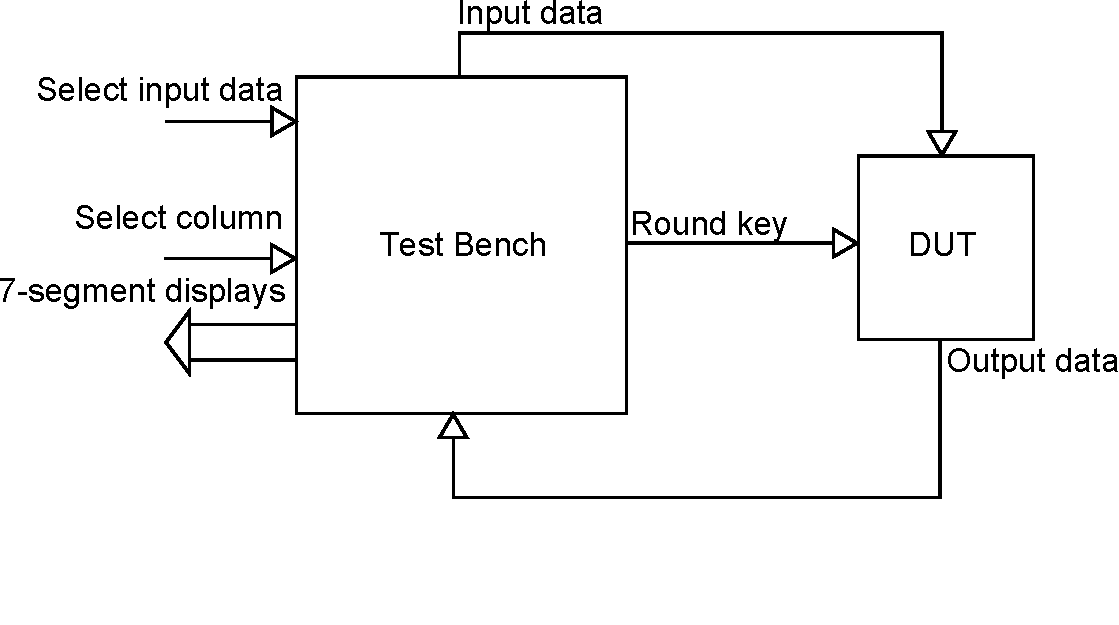
\includegraphics[width=\linewidth]{test_bench}
\caption{Test bench overview}
\label{fig:test bench overview}
\end{figure}

\end{document}
